\documentclass[12pt]{article}
\usepackage[margin=1in]{geometry}
\usepackage{setspace}
\onehalfspacing

% Start of preamble
%==========================================================================================%
% Required to support mathematical unicode
\usepackage[warnunknown, fasterrors, mathletters]{ucs}
\usepackage[utf8x]{inputenc}

\usepackage[dvipsnames,table,xcdraw]{xcolor} % colors
\usepackage{hyperref} % links
\hypersetup{
	colorlinks=true,
	linkcolor=blue,
	filecolor=magenta,      
	urlcolor=cyan,
	pdfpagemode=FullScreen
}

% Standard mathematical typesetting packages
\usepackage{amsmath,amssymb,amscd,amsthm,amsxtra, pxfonts}
\usepackage{mathtools,mathrsfs,dsfont,xparse}

% Symbol and utility packages
\usepackage{cancel, textcomp}
\usepackage[mathscr]{euscript}
\usepackage[nointegrals]{wasysym}
\usepackage{apacite}

% Extras
\usepackage{physics}  % Lots of useful shortcuts and macros
\usepackage{tikz-cd}  % For drawing commutative diagrams easily
\usepackage{microtype}  % Minature font tweaks

\usepackage{enumitem}
\usepackage{titling}

\usepackage{graphicx}
\usepackage{wrapfig}

% Fancy theorems due to @intuitively on discord
\usepackage{mdframed}
\newmdtheoremenv[
backgroundcolor=NavyBlue!30,
linewidth=2pt,
linecolor=NavyBlue,
topline=false,
bottomline=false,
rightline=false,
innertopmargin=10pt,
innerbottommargin=10pt,
innerrightmargin=10pt,
innerleftmargin=10pt,
skipabove=\baselineskip,
skipbelow=\baselineskip
]{mytheorem}{Theorem}

\newenvironment{theorem}{\begin{mytheorem}}{\end{mytheorem}}

\newmdtheoremenv[
backgroundcolor=BurntOrange!30,
linewidth=2pt,
linecolor=BurntOrange,
topline=false,
bottomline=false,
rightline=false,
innertopmargin=10pt,
innerbottommargin=10pt,
innerrightmargin=10pt,
innerleftmargin=10pt,
skipabove=\baselineskip,
skipbelow=\baselineskip
]{mycorollary}{Corollary}

\newenvironment{corollary}{\begin{mycorollary}}{\end{mycorollary}}


\newmdtheoremenv[
backgroundcolor=OrangeRed!30,
linewidth=2pt,
linecolor=OrangeRed,
topline=false,
bottomline=false,
rightline=false,
innertopmargin=10pt,
innerbottommargin=10pt,
innerrightmargin=10pt,
innerleftmargin=10pt,
skipabove=\baselineskip,
skipbelow=\baselineskip
]{mylemma}{Lemma}

\newenvironment{lemma}{\begin{mylemma}}{\end{mylemma}}

\newtheoremstyle{definitionstyle}
	{\topsep}%
	{\topsep}%
	{}%
	{}%
	{\bfseries}%
	{.}%
	{.5em}%
	{}%
\theoremstyle{definitionstyle}
\newmdtheoremenv[
backgroundcolor=Violet!30,
linewidth=2pt,
linecolor=Violet,
topline=false,
bottomline=false,
rightline=false,
innertopmargin=10pt,
innerbottommargin=10pt,
innerrightmargin=10pt,
innerleftmargin=10pt,
skipabove=\baselineskip,
skipbelow=\baselineskip,
]{mydef}{Definition}
\newenvironment{definition}{\begin{mydef}}{\end{mydef}}

\newtheorem*{remark}{Remark}

\newtheorem*{example}{Example}

% Common shortcuts
\def\mbb#1{\mathbb{#1}}
\def\mfk#1{\mathfrak{#1}}

\def\bN{\mbb{N}}
\def \C{\mbb{C}}
\def \R{\mbb{R}}
\def\bQ{\mbb{Q}}
\def\bZ{\mbb{Z}}
\def \cph{\varphi}
\renewcommand{\th}{\theta}
\def \ve{\varepsilon}
\newcommand{\mg}[1]{\| #1 \|}

% Sometimes helpful macros
\newcommand{\floor}[1]{\left\lfloor#1\right\rfloor}
\newcommand{\ceil}[1]{\left\lceil#1\right\rceil}
\renewcommand{\qed}{\hfill\qedsymbol}
\renewcommand{\H}{\mbb H}
\renewcommand{\S}{\mbb S}

% Sets
\usepackage{braket}

% End of preamble
%==========================================================================================%

% Start of commands specific to this file
%==========================================================================================%

\renewcommand{\ip}[2]{\langle #1, #2 \rangle}
\newcommand{\linf}[1]{\max_{1\leq i \leq #1}}
\newcommand{\seq}[2]{\qty(#1_#2)_{#2=1}^{\infty}}

%==========================================================================================%
% End of commands specific to this file

\title{The nicest space of them all: $\overline \C \cong \S^2$ and it's circle-preserving homeomorphisms}
\date{\today}
\author{Anonymous}

\begin{document}

\maketitle
	
	\begin{abstract}
		In this paper we give all the necessary background knowledge to understand both the concepts and the proof of the theorem involving circle-preserving homeomorphisms.
	\end{abstract}

	We shall work towards proving the following theorem:
	\begin{theorem}
		$f$ is a circle preserving homeomorphism of $\overline \C$ if and only if $f$ is a Möbius transformation or the composition of complex conjugation with a Möbius transformation.
	\end{theorem}
	This is quite the spectacular theorem. From simply sending circles to circles, one can deduce precisely the type of map this homeomorphism will be. 
	
	\section{Defining the Riemann sphere}
	Formally, the Riemann sphere is the one-point-compactification of $\C$. To define this, we need the following:
	\begin{definition}
		A space $X$ is said to be locally compact at $x$ if there exists a compact subspace $C$ of $X$ that contains a neighborhood of $X$. If $X$ is locally compact at each of its points, $X$ is said to be locally compact.
	\end{definition}
	We guide the reader to section 29 of Munkres for the proof of the following theorem:
	\begin{theorem}
		Let $X$ be a space. Then $X$ is locally compact Hausdorff if and only if there exists a space $Y$ satisfying the following conditions:
		\begin{enumerate}
			\item $X$ is a subspace of $Y$.
			\item The set $Y - X$ consists of a single point.
			\item $Y$ is a compact Hausdorff space.
		\end{enumerate}
		If $Y$ and $Y'$ are two spaces satisfying these conditions, then there is a homeomorphism of $Y$ with $Y'$ that equals the identity map on $X$.
	\end{theorem}
	
	The topology $Y$ is constructed as follows:
	\begin{align*}
		\mathcal{T} = \mathcal{T_X} \cup \set{Y - C | C \subset X \text{ compact }}
	\end{align*}
	For example, $\overline{\C} \setminus \overline{B_1}(0)$ is an open subset of $\overline{\C}$. Next, we prove exercise 5 in the aforementioned section of Munkres, that is
	\begin{theorem}
		If $f: X_1 \to X_2$ is a homeomorphism of locally compact Hausdorff spaces, then $f$ extends to a homeomorphism of their one-point compactifications.
	\end{theorem}
	\begin{proof}
		Let $Y_1 = X_1 \cup \set{p},\; Y_2 = X_2 \cup \set{q}$ denote the one-point compactification of $X_1,\; X_2$ respectively. Define $\tilde{f}(x) = f(x)$ for $x \in X_1$, and $f(p) = q$. For any open set $U \subset Y_2$, if $q \not \in U$ then $\tilde{f}^{-1}(U) = f^{-1}(U)$ which is an open subset of $X_1$, and by how we defined the topology on $Y_1$, it too is an open subset of $Y_1$. If $q$ is in $U$, then $Y_2 \setminus U = C \subset X_2$ is compact. Thus $\tilde{f}^{-1}(C) = f^{-1}(C)$ is compact (since $f$ is a homeomorphism, its inverse is continuous). Thus $\tilde f^{-1}(U) = Y_1 \setminus \tilde f^{-1}(C)$ is open in $Y_1$, since it is the complement of a compact set in $X_1$. By running the exact same argument for the inverse map, we have proven the theorem.
	\end{proof}

	\section{$\overline{\C} \cong \S^2$}
	We have seen the homeomorphism from $\S^1 \setminus \set{(0, 1)}$ to $\R$ previously on homework 4. The idea of a one-point-compactification is fascinating in its own way. However, by extending this idea from the first to the second dimension, we can produce much more interesting results, that don't have immediate analogues in the first dimension (For example, what would be a circle on the circle? On the other hand, a circle on the sphere is well understood and barely merits a definition). The incredible idea of stereographic projection works here as well. Define $\pi: \S^2 \setminus \Set{(0,0,1)} \to \C$ by 
	\begin{align*}
		\pi(x_1, x_1, x_1) = \frac{x_1+ix_2}{1-x_3}
	\end{align*}
	\begin{wrapfigure}{r}{0.33\textwidth} %this figure will be at the right
		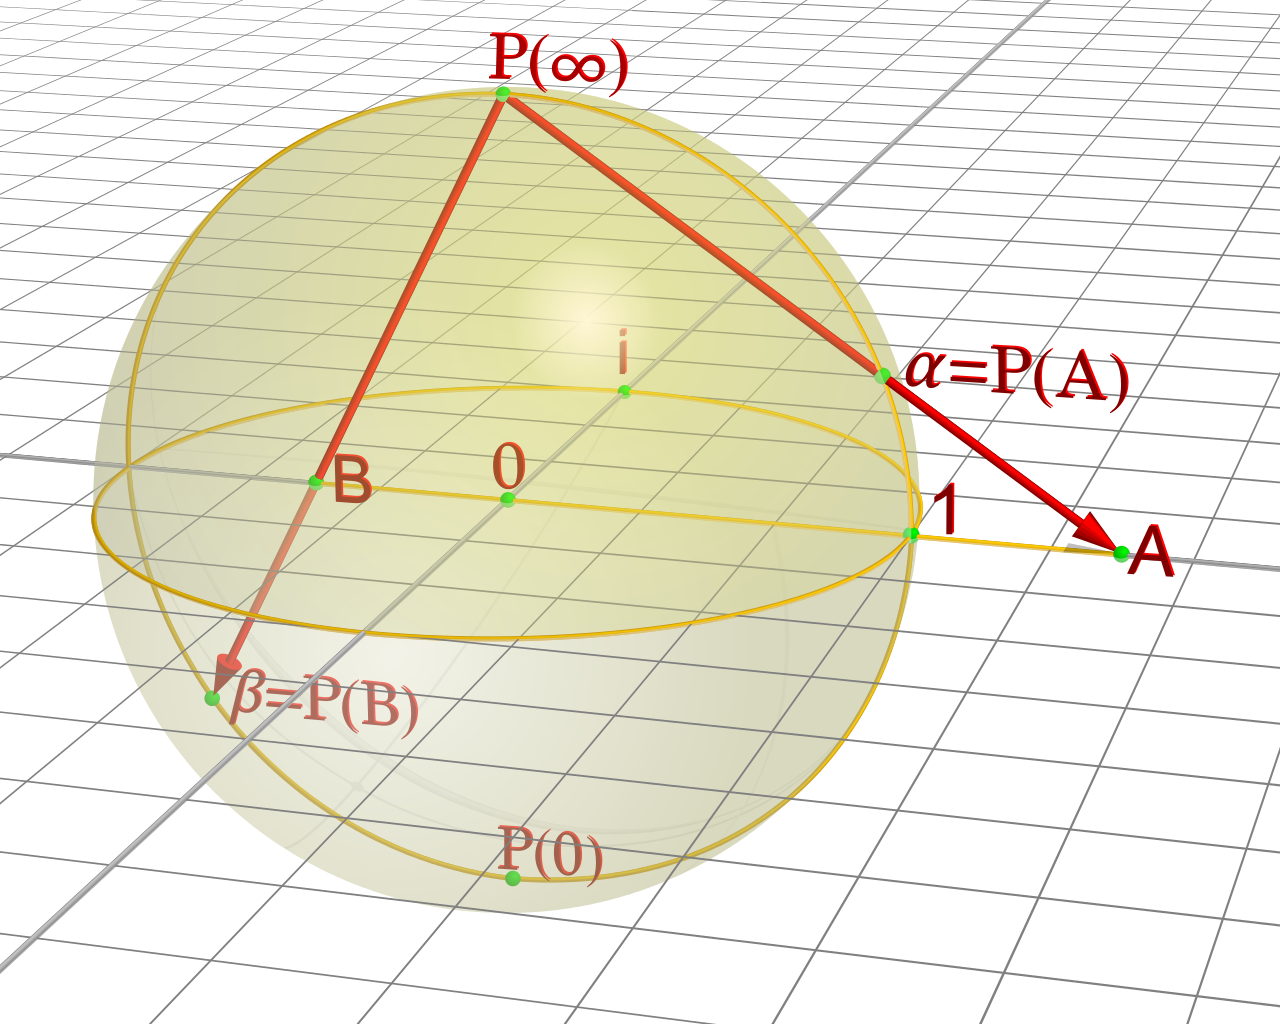
\includegraphics[width=0.33\textwidth]{projection}
	\end{wrapfigure}

	
	\begin{wrapfigure}{r}{0.25\textwidth} %this figure will be at the right
		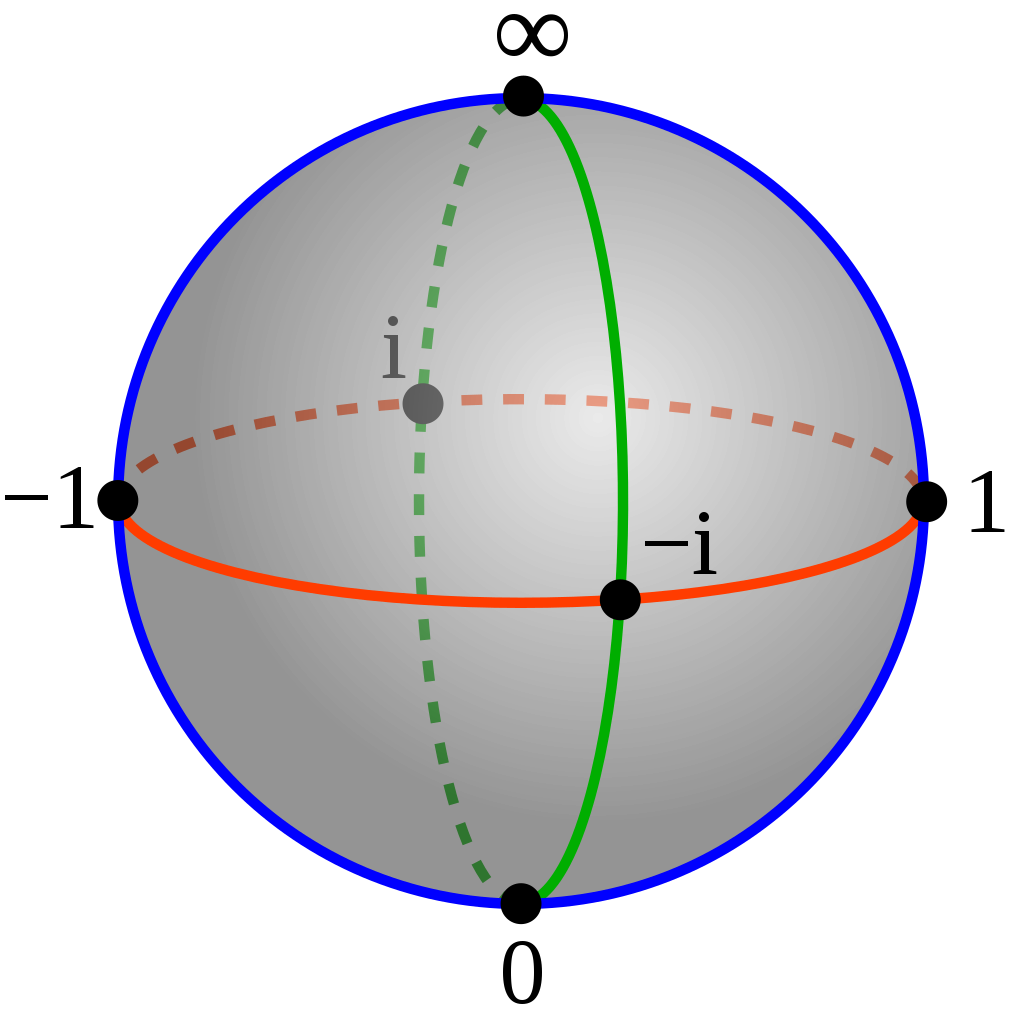
\includegraphics[width=0.25\textwidth, height=3.8cm]{riemannsphere}
	\end{wrapfigure}
	If $z = x+iy \in \C$, the inverse function is given by \begin{align*}
		x_1 = \frac{2x}{x^2+y^2+1}, \quad x_2 = \frac{2y}{x^2+y^2+1}, \quad x_3 = \frac{x^2+y^2-1}{x^2+y^2+1}
	\end{align*}
	which the reader may find a proof of on page 2 of \cite{complex}. Note that $\pi$ and $\pi^{-1}$ are the ratio of polynomials in each entry from $\S^2 \to \C$ and $\C \to \S^2$ (resp.), who's denominator is never 0, and hence are both continuous.
	
	As $\S^2$ is clearly the one-point-compactification of $\S^2 \setminus \Set{(0, 0, 1)}$, by our definition of $\overline{\C}$ as the one-point-compactification of $\C$, the previous theorem lets us extend this homeomorphism to a homeomorphism of the sphere with the extended complex plane. For this reason the extended complex plane is often called the Riemann sphere. A lot of intuition comes from having this picture in mind. We struggle to understand the concept of going infinitely out on the complex plane. However, it is much easier to understand a point sitting up above a 2d plane, and curving the plane to ``converge'' in a sense at that point. The following picture demonstrates precisely that idea, and can help us visualize some (at first) seemingly bizarre properties.
	
	For example, since $\S^2$ is sequentially compact, every sequence has a convergent subsequence. We propose a question to the reader: what is a convergent subsequence of $(n)_{n \in \bN} \subset \overline{\C}$? Itself! If one lets $\infty \coloneqq \pi(0, 0, 1)$ (visualized above), we have that $(n)_{n \in \bN} \to \infty$, which may be visualized as wrapping along the right side of the Riemann sphere. (This is proved by a fact mentioned in Theorem 4 below.) Also, the extended real line $\R \cup \Set{\infty}$ can be visualized as the blue circle on the above picture, which notably is a circle on the sphere.
	
	\section{Arithmetic in $\overline{\C}$}
	For the sake of being concise when defining functions, we provide here some basic arithmetic on $\overline \C$. Define the following:
	\begin{align*}
		&z + \infty = \infty \text{ for all $z \in \C$,}\\
		&z \times \infty = \infty \text{ for all $z \in \C$,}\\
		&\frac{z}0 = \infty \text{ and } \frac{z}{\infty} = 0 \text{ for all $z \in \C \setminus \Set{0}$}
	\end{align*}
	with $\infty \times \infty = \infty$, while $\infty - \infty$ and $0 \times \infty$ are left undefined. Similarly, let $\infty/0 = \infty$, $0/\infty = 0$, and leave $\infty/\infty$ and $0/0$ undefined. With these definitions $\overline{\C}$ does not define a field, as $\infty$ does not have an additive inverse. All of these definitions should feel rather intuitive, except perhaps that $z/0 = \infty$ for nonzero $z$. The reader recalls that $\lim_{z \to 0} 1/z$ doesn't exist since it tends to $-\infty$ on the left and $+\infty$ on the right. Here these infinities are treated as one and the same, which is why we can make this definition. It also turns out that the most important one is $z/0 = \infty$ for $z \neq 0$, and the reader should carefully remember this.
	
	\section{Möbius Transformations}
	A Möbius transformation is a map from $\overline{\C} \to \overline{\C}$ of the form
	\begin{align*}
		f(z) = \frac{az+b}{cz+d}, \; a, b, c, d \in \C, \; \text{ with } ad -  bc \neq 0.
	\end{align*}
	For polynomials $p(z), q(z)$, if $g(z) = p(z)/q(z)$ define $g(\infty) = \lim_{z \to \infty} g(z)$. For a Möbius transformations $f$ as above, $f(\infty)$ always exists, since it is $a/c$ if $c \neq 0$ and $\infty$ if $c = 0$.
	The reader should recall that we claimed that these were all circle-preserving homeomorphisms. In particular, they were all homeomorphisms, which of course implies bijective. Indeed, if $f$ is as above, then $f$ has inverse
	\begin{align*}
		f^{-1}(z) = \frac{dz-b}{-cz+a}.
	\end{align*}
	A proof that this is true may be found in \cite{bijective}.
	
	From here we claim that these Möbius transformations are continuous on the Riemann sphere. This is quite valuable as one should note that we must show that Möbius transformations are continuous with continuous inverses. Also notice that if we can show Möbius transformations are continuous, since their inverse is also a Möbius transformation, we will immediately have that they are homeomorphisms. 
	
	
	\begin{theorem}
		If $f(z) = p(z)/q(z)$ where $p$ and $q$ are polynomials which share no common roots, then $f: \overline \C \to \overline \C$ is continuous.
	\end{theorem}
	\begin{proof}
		We must show that, given any $w \in \Sigma$, and any sequence $z_n \to w$, then $f(z_n) \to f(w)$. First, we claim that $z_n \to \infty$ (in the topological sense) iff $|z_n| \to \infty$ with $|\infty| = \infty$ (in the real analysis sense). Let's start with the reverse direction. 
		
		We must show that if $|z_n| \to \infty$, then for any neighborhood $V = \Sigma \setminus K$, $K$ compact of $\infty$, all but finitely many of the $z_n$'s lie in $V$. Since $K$ is compact by Heine-Borel it is bounded, say by $M$. By definition of a limit we can find $N$ sufficiently large so that if $n \geq N$, $|z_n| \geq M$. Thus $z_n \in V$ for all $n \geq N$, proving this direction.
		
		For the reverse direction, assume that for any neighborhood $V = \Sigma \setminus K$ of $\infty$, where $K$ is compact, we have that all but finitely many of the $z_n$'s are in $V$. Now let $M > 0$ be arbitrary. Since $\Sigma \setminus \overline{B_0}(M)$ is a neighborhood of $\infty$, we have that all but finitely many of the $z_n$'s lie in this neighborhood. That is, there is some $N \geq 0$ so that if $n \geq N$, $z_n \in \Sigma \setminus \overline{B_0}(M)$, which is what we wanted to show.
		
		From the first paragraph, suppose that $w \neq \infty$. Topologically we can find $N$ sufficiently large so that all but finitely many of the $z_n$'s lie in $B_1(w)$, and in particular are not infinity. We have two cases:
		\begin{enumerate}[label=(\arabic*)]
			\item $f(w) \in \C$. In this case, since $f(z)$ restricted to $\C$ is the quotient of two linear polynomials, who's denominator is not 0 at the point $w$, we may conclude that that $f$ is continuous there.
			\item $f(w) = \infty$. Then $q(w) = 0$ and $p(w) \neq 0$ (by coprimality). So $|p(w)| \geq 2\ve$ for some small $\ve$, and thus we can find a neighborhood of $w$ so that $|p(z)| \geq \ve$ for $z$ in that neighborhood. Now, by the above equivalence, for any $M > 0$, we must produce a $\delta > 0$ so that if $0 < |z_n - w| < \delta$, $|f(w)| \geq M$ to complete the proof. By the continuity of the polynomial $q$, we may find $\delta$ (sufficiently small) so that $|q(z)| \leq \ve/M$. Then for any $0 < |z_n-w| < \delta$, $|p(z)/q(z)| \geq \ve \cdot M/\ve = M$.
		\end{enumerate}
		Finally, we defined $f(\infty) = \lim_{z \to \infty} f(z)$. By what we know from analysis, if $|z_n| \to \infty$, then $\lim_{n \to \infty} f(z_n) = \lim_{z \to \infty} f(z) = f(\infty)$ (Notice that if $z_n = \infty$, then $f(z_n) = f(\infty)$), so we have guaranteed continuity at $\infty$, and we are done.
	\end{proof}
	
	To be a Möbius transformation, the top and bottom linear polynomial must not share a root or they would cancel to a constant and not be injective. So, this shows that Möbius transformations are continuous, and hence homeomorphisms. Now we would like to give the reader greater intuition for this incredibly special class of functions, by describing what generates them.
	
	\begin{lemma}
		Every Möbius transformation is the composition of
		\begin{enumerate}[label=(\roman*)]
			\item Transformations of the form $e^{i\theta} z$ ($\theta \in \R$),
			\item The transformation $z \mapsto z^{-1}$, representing a rotation by the angle $\pi$ about the axis through $\pm 1$ on $\S^2$,
			\item The transformations $z \mapsto rz$, $r \in \R_{>0}$ (stretching),
			\item The transformations $z \mapsto z + t$, $(t \in \C)$ (translations).
		\end{enumerate}
	\end{lemma}
	\begin{proof}[Proof \cite{complex}.]
		First we note here that all Möbius transformations may be changed so that $ad-bc = 1$. Indeed, if
		\begin{align*}
			T(z) = \frac{az+b}{cz+d}
		\end{align*}
		We see that
		\begin{align*}
			T(z) = \frac{a/(\sqrt{ad-bc})z + b/(\sqrt{ad-bc})}{c/(\sqrt{ad-bc})z + d/(\sqrt{ad-bc})}
		\end{align*}
		And hence the ``new'' $ad-bc = a/(\sqrt{ad-bc})d/(\sqrt{ad-bc}) - b/(\sqrt{ad-bc})c/(\sqrt{ad-bc}) = (ad-bc)/(ad-bc) = 1$.
		
		
		So now, letting $T$ be a Möbius transformation with $ad-bc = 1$, if $c = 0$ then $T(z) = (az+b)/d$ with $a, d \neq 0$ so let $a/d = re^{i\theta}$ and $b/d = t$. Then $T(z) = re^{i\theta} + t$, so
		\[\begin{tikzcd}
			{\overline \C} && {\overline \C} && {\overline \C} && {\overline \C}
			\arrow["{z \mapsto e^{i\theta}z}", from=1-1, to=1-3]
			\arrow["{z \mapsto rz}", from=1-3, to=1-5]
			\arrow["{z \mapsto z + t}", from=1-5, to=1-7]
			\arrow["T"', bend left, from=1-1, to=1-7]
		\end{tikzcd}\]
	
		If $c \neq 0$, then letting $T_{a/c}(z) = z+a/c$, and $J(z) = z^{-1}$, one sees that
		
		\begin{align*}
			T(z) &= \frac ac - \frac{1}{c(cz+d)} \\
			&= (T_{a/c} \circ J)(-c^2z-cd)
		\end{align*}
		and by the above, we see that $-c^2z-cd$ can be expressed in terms of the above generators, thus $T$ can as well.
	\end{proof}

	Now we have reached the heart and soul of the paper. We are finally ready to talk about circle-preserving homeomorphisms. We have seen that Möbius transformations are continuous with continuous inverses (which is also a Möbius transformation). We need to now first define what a circle is, show that Möbius transformations preserve them, and finally, show that only the Möbius transformations (perhaps composed with complex conjugation) preserve them.
	\begin{definition}
		A circle in the sphere $\S^2 \subset \R^3$ is the intersection $\S^2 \cap \Pi$ where $\Pi$ is a plane in $\R^3$ that is intersecting and not tangent to $\S^2$. A circle in $\overline \C$ is thus the image of this set under the prescribed homeomorphism.
	\end{definition}
	A long calculation which one may find in \cite{complex} shows that if $\alpha x_1 + \beta x_2 + \gamma x_3 = \delta$ ($\alpha, \beta, \gamma \in \R$) is a plane corresponding to the circle $C$ in $\S^2$, then $C$ is given by the equation $2\alpha \Re(z) + 2 \beta \Im(z) + \gamma(|z|^2-1) = \delta(|z|^2+1)$. Referencing the book, this leads to there being two types of circles: regular Euclidean circles in $\C$, and Euclidean straight lines in $\C$ along with $\infty$ (which, on the Riemann sphere, is of course still a circle, as for example the reader recalls how the extended real line was visualized!) The reader at this point should not be surprised that Möbius transformations do in fact preserve circles.
	
	\begin{theorem}
		If $C$ is a circle of $\overline \C$, and if $T$ is a Möbius transformation, then $T(C)$ is a circle of $\overline \C$.
	\end{theorem}
	\begin{proof}
		First, as the map $z \mapsto z^{-1}$ induces a rotation by an angle $\pi$ about the axis going through $\pm 1$ on the sphere (See section 1.3 of \cite{complex}), and as this action on a circle clearly yields a circle, the map $z\mapsto z^{-1}$ preserves circles. For the rest, we have two cases:
		
		For euclidean circles:
		\begin{enumerate}[label=(\roman*)]
			\item For circles of the form $(x-a)^2 + (y-b)^2 = R^2$, one sees that the map $x+iy \mapsto x\cos(\theta)-y\sin(\theta)+i(x\sin(\theta)+y\cos(\theta))$ yields
			\begin{align*}
				(x\cos(\theta)-y\sin(\theta)-a)^2 + (x\sin(\theta)+y\cos(\theta)-b)^2 &= R^2 \iff \\
				x^2-x2(a\cos(\theta)+b\sin(\theta)) + b^2 + y^2 +y2(a\sin(\theta)-b\cos(\theta)) + a^2 &= R^2
			\end{align*}
			Now, from the identity $(a \cos(\theta)+b \sin(\theta))^2+(a\sin(\theta)-b\cos(\theta))^2 = a^2+b^2$, we see we do not need to add anything to complete the square, and thus our circle is
			\begin{align*}
				(x-(a\cos(\theta)+b\sin(\theta))^2 + (y+(a\sin(\theta)-b\cos(\theta))^2 = R^2
			\end{align*}
			This is of course what we expected, as the center $(a, b)$ under the aforementioned transformation gets mapped there.
			
			\item For $z \mapsto rz$, we would get 
			\begin{align*}
				(rx-a)^2 + (ry-b)^2 &= R^2 \iff \\
				(x-a/r)^2 + (y-b/r)^2 &= (R/r)^2
			\end{align*}
			\item The translation $z \mapsto z+(c+id)$ is similar.
		\end{enumerate}
		For circles of the form $\Lambda \cup \Set{\infty}$ where $\Lambda$ is a straight line in $\C$, the default equation is $y = mx + b$. Thus,
		\begin{enumerate}[label=(\roman*)]
			\item The transformation $x+iy \mapsto x\cos(\theta)-y\sin(\theta)+i(x\sin(\theta)+y\cos(\theta))$ gives
			\begin{align*}
				x\sin(\theta)+y\cos(\theta) = m(x\cos(\theta)-y\sin(\theta)) + b \\
				x(\sin(\theta)-m\cos(\theta)) + y(\cos(\theta)+m\sin(\theta)) = b
			\end{align*}
			Which is clearly seen to be a (possibly vertical) line. 
			
			\item The transformation $x+iy \mapsto rx + iry$ yields
			\begin{align*}
				ry = mrx + b \iff y = mx + b/r
			\end{align*}
			Again clearly a line. Finally,
			\item The translation $x + iy \mapsto x + iy + (c+id)$ is clear like last time. 
		\end{enumerate}
	
		By the lemma every Möbius transformation is a composition of these. Since each of these maps circles to circles, the theorem has been proved.
	\end{proof}
	
	Finally, to complete the forward direction of the theorem we are working towards, we give this theorem:
	\begin{theorem}
		The map $z \mapsto \overline{z}$ with the added condition that $\overline{\infty} = \infty$, who's inverse is itself, is a circle-preserving homeomorphism. 
	\end{theorem}
	\begin{proof}
		Exercise.
	\end{proof}
	
	\section{The Reverse Implication}
	Recall that the theorem we are trying to prove is
	\begin{theorem}
		$f$ is a circle preserving homeomorphism of $\overline \C$ if and only if $f$ is a Möbius transformation or the composition of complex conjugation with a Möbius transformation.
	\end{theorem}
	
	We just finished the proof of the forward implication in the last section. The reverse direction is signifigantly harder to prove, and requires some lemmas. First, we give some motivation. This theorem gives rise to a very large class of homeomorphisms of $\overline \C$, which is topologically important. This theorem is of particular importance to us since it takes a relatively simple condition (preserving circles) to specify exactly what type of map the homeomorphism will be. A similar statement is true for hyperbolic geometry which we will not discuss, but the interested reader may look into more in \cite{complex}.
	
	To begin the proof, we need a few lemmata:
	\begin{lemma}
		If $m(z)$ fixes three distinct points of $\overline \C$, then $m(z)$ is the identity.
	\end{lemma}
	\begin{proof}
		If $m(\infty) = \infty$, then $c = 0$. This yields $m(z) = az + b$ for some $a,  b$. Fixing two points means that the linear polynomial $(a-1)z + b = 0$ has two solutions, which can only happen if $a = 1$ and $b = 0$. Similarly, if $c \neq 0$, then $m(\infty) \neq \infty$. So all three fixed points lie in $\C$. Notice that 
		\begin{align*}
			\frac{az+b}{cz+d} = z \iff az+b = cz^2 + dz \iff cz^2 + z(d-a) - b = 0
		\end{align*}
		is a quadratic. To have three roots, this quadratic must be equivalently 0, that is, $c = 0$, $d = a$, and $b = 0$, which is again the identity.
	\end{proof}
	\begin{lemma}
		There is a unique Möbius transformation sending $(z_1, z_2, z_3)$ to $(w_1, w_2, w_3)$.
	\end{lemma}
	\begin{proof}
		(Uniqueness) Let $m$ and $n$ be Möbius transformations doing the above. Then $n^{-1} m$ is a Möbius transformation fixing three points and hence is the identity.
		
		
		(Existence)
		When all the $z_1, z_2, z_3$ lie in $\C$, the map
		\begin{align*}
			m(z) = \frac{z-z_1}{z-Z_3} \frac{z_2-z_3}{z_2-z_1} = \frac{(z_2-z_3)z - z_1(z_2-z_3)}{(z_2-z_1)z - z_3(z_2-z_1)}
		\end{align*}
		sends $(z_1, z_2, z_3)$ to $(0, 1, \infty)$ by plugging things in, and is Möbius since $ad-bc = (z_2-z_3)(-z_3)(z_2-z_1) - (-z_1)(z_2-z_3)(z_2-z_1) = (z_2-z_3)(z_1-z_3)(z_2-z_1)$ which is nonzero since the $z_i$'s are distinct. For the map sending $(\infty, z_2, z_3)$ to $(0, 1, \infty)$, the function
		\begin{align*}
			m(z) = \frac{z_2-z_3}{z-z_3}
		\end{align*}
		works. The case $\infty \mapsto \infty$ results in picking $c = 0$, and is so simple we leave it as an exercise to the reader. Now, let $m$ be the map sending $(z_1, z_2, z_3)$ to $(0, 1, \infty)$, and let $n$ be the map sending $(w_1, w_2, w_3)$ to $(0, 1, \infty)$. The map $n^{-1} m$ is the desired map, and the theorem has been proved.
	\end{proof}
	We reference the book in that three distinct points in $\overline \C$ uniquely identify a circle (or a line, if one of the points is $\infty$). The reader might intuitively see this because two linear independent vectors span precisely 1 plane, so specifying 3 noncollinear points on the sphere will specify a unique plane, and (by definition) yield a unique circle.
	
	\begin{proof}[Proof Of The Reverse Implication.]
		The book gives a sketch of this proof. We attempt here to complete and improve the proof. We have already seen that all of those maps are circle-preserving homeomorphisms. We must prove the other direction. Let $f$ be a circle-preserving homeomorphism, and let $p$ be the Möbius transformation sending $(f(0), f(1), f(\infty))$ to $(0, 1, \infty)$, so $p \circ f$ satisfies $p \circ f(0) = 0$, $p \circ f(1) = 1$, and $p \circ f(\infty) = \infty$. $\overline \R$ (the extended real line) is the unique circle determined by $(0, 1, \infty)$, and thus $f(\overline \R) = \overline \R$.
		
	 	We claim that $p \circ f (\mbb H)$ is either the upper-half or the lower-half plane. Notice that nothing in this image can lie on the extended real line by bijectivity. Case 1: there is some $z \in \mbb H$ so that $p \circ f (z) \in \mbb H$. Now suppose that there was some $w \in \mbb H$ so that $p \circ f(w)$ had negative imaginary part. Letting $\Lambda$ be the straight line connecting $z$ to $w$, $\Lambda$ is connected while $(p \circ f(\Lambda) \cap \mbb H, p \circ f(\Lambda) \cap -\mbb H)$ forms a disconnection of the image, a contradiction. Suppose, with the previous conditions still holding, there was some $a \in - \mbb H$ so that $p \circ f(a)$ had positive real part. The segment connecting $f(z)$ to $f(a)$ is connected but it's preimage is not, which contradicts $p \circ f$ being a homeomorphism. Since $f$ is onto this shows that $f(\overline \H) = \overline \H$ in this case. The other case is extremely similar and is left as an exercise to the reader, so the only other possibility is that $f(\overline \H) = -\mbb \H)$. 
		
		In the first case set $m = p$, and in the second set $m = C \circ p$, where $C$ is complex conjugation. This yields a map preserving the upper half plane, and sending $(0, 1, \infty)$ to itself. One sees that $m \circ f$ sends Euclidean circles to Euclidean circles, and Euclidean lines to Euclidean lines, as in the first case you cannot pick up $\infty$, and in the second you cannot lose $\infty$. Let $Z$ denote the set of fixed points of $m \circ f$. We claim that if $X, Y$ are two circles (as in definition 2) in $\C$ that intersect at $z_0$, with $m \circ f(X) = X$ and $m \circ f(Y) = Y$, then $m \circ f(z_0) = z_0$. This follows since $f$ is injective thus $f(\Set{z_0}) = f(X \cap Y) = f(X) \cap f(Y) = X \cap Y = \Set{z_0}$.
		
		For each $s \in \R$, let $V(s)$ be the vertical line in $\C$ through $s$ and let $H(s)$ be the vertical line in $\C$ through $is$.
		
		Let $H$ be any horizontal line in $\C$ that is not $\R$. As $m \circ f(\R) = \R$ and $H,\; \R$ are disjoint, $m \circ f(H)$ and $m \circ f(\R) = \R$ are disjoint lines in $\C$, so $H$ is a horizontal line $\C$. As $m \circ f(\H) = \H$, $H$ lies in $\H$ iff $m \circ f(H)$ lies in $\H$.
		
		Let $A$ denote the Euclidean circle with Euclidean center 1/2 and radius 1/2. As $V(0)$ is tangent (in the geometrical sense) to $A$ at 0, we see that $m \circ f(V(0))$ is tangent to $m \circ f(A)$ at $m \circ f(0) = 0$, since $m \circ f(A \cap V(0)) = (m \circ f(A)) \cap (m \circ f(V(0))$ by injectivity. Similarly $m \circ f(V(1))$ is the tangent line to $m \circ f(A)$ at 1.
		
		As $V(0)$ and $V(1)$ are parallel lines in $\C$, $m \circ f(V(0))$ and $m \circ f(V(1))$ are also parallel lines in $\C$ (by the same injectivity argument), and by rotational symmetry of the complex plane, our arguments showing that if $H$ is horizontal then $H$ lies in $\mbb H$ iff $m \circ f(H)$ lies in $\mbb H$, we can conclude that if $V$ is vertical, then $V$ lies in the right half of the complex plane iff $m \circ f(V)$ lies in the right half of the complex plane. Necessarily then $m \circ f(V(1))$ is a vertical line going through 1 and is hence $V(1)$, and by being parallel with $f(0) = 0$, $m \circ f(V(0)) = V(0)$.
		
		This forces $f(A) = A$, as the tangent lines through 0 and 1 of any other Euclidean circle passing through 0 and 1 are not parallel. One may see this by seeing that if $(x-a)^2+(y-b)^2 = r^2$, and 0 and 1 lie on this circle, then $a^2 + b^2 = r^2$, and $(1-a)^2 + b^2 = r^2$, yielding $a^2 - (1-a)^2 = 0$, which says that $a=1/2$. An explicit calculation shows that $r \geq 1$, and that if $r > 1$ the above claim holds. Even though $m \circ f(A) = A$, we do not know that $A$ contains any points of $Z$ other than 0 and 1.
		
		So we run the same argument with the two horizontal tangent lines to $A$. Considering the first tangent $H(1/2)$ to $A$ at $1/2 + 1/2 i$, we see that $m \circ f(H(1/2))$ is again a horizontal line in $\H$ tangent to $m \circ f(A)$, and so $m \circ f(H(1/2)) = H(1/2)$ ($A$ has only one tangent line that is horizontal in the upper half plane). This gives more points in $Z$, such as the intersection of the above horizontal and vertical lines, i.e. the points $1/2i$ and $1 + 1/2 i$. Running the same argument on $H(-1/2)$ yields that the points $-1/2i$ and $1 - 1/2i$ lie in $Z$. 
		
		By running this exact same argument on the circle centered at $x > 0$ with radius $x$, as $(0, x), (0, -x), (2x, x)$ and $(2x, -x)$ are clearly the four ``corners'' of the circle, we get that $\Set{x + iy | y = \pm \frac12 x, \; x \geq 0} \subset Z$ as well.
		
		
		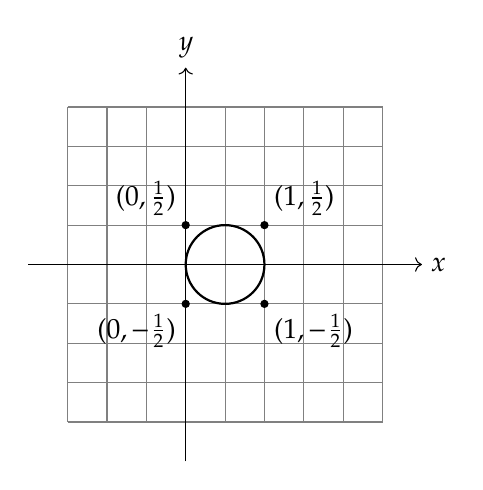
\begin{tikzpicture}
			
			\draw[step=0.5,gray,thin] (-1.5,-2) grid (2.5,2);
			\draw[->] (-2,0) -- (3,0) node[right] {$x$};
			\draw[->] (0,-2.5) -- (0,2.5) node[above] {$y$};
			
			% Draw the circle
			\draw[thick] (1/2, 0) circle [radius=1/2];
			
			% Label the points
			\fill (0,1/2) circle [radius=1.5pt] node[above left] {$(0,\frac{1}{2})$};
			\fill (1,1/2) circle [radius=1.5pt] node[above right] {$(1,\frac{1}{2})$};
			\fill (1,-1/2) circle [radius=1.5pt] node[below right] {$(1,-\frac{1}{2})$};
			\fill (0, -1/2) circle [radius=1.5pt] node[below left] {$(0,-\frac{1}{2})$};
			
		\end{tikzpicture}
		$\quad \quad \quad \quad \quad \quad \quad \quad \quad$
		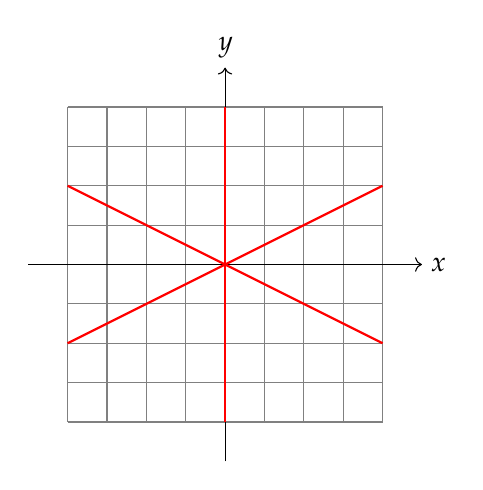
\begin{tikzpicture}
			\draw[step=0.5,gray,thin] (-2,-2) grid (2,2);
			\draw[->] (-2.5,0) -- (2.5,0) node[right] {$x$};
			\draw[->] (0,-2.5) -- (0,2.5) node[above] {$y$};
			
			% Line segments
			\draw[thick, red] (0,0) -- (2,1);
			\draw[thick, red] (0,0) -- (2,-1);
			\draw[thick, red] (0, -2) -- (0, 2);
			\draw[thick, red] (0,0) -- (-2,1);
			\draw[thick, red] (0,0) -- (-2,-1);
		\end{tikzpicture}
		
		The final part of this proof that we give is separate from the one in the book, but we find this both more intuitive and cleaner. One notes that all our arguments didn't depend on $x > 0$, so indeed, we can run the same argument to get that $\Set{x+iy | y=\pm \frac12 x,\; x \leq 0} \subset Z$ as well (visualized as the left half of the red picture). Now, let $z_0 = x_0 + iy_0$ lie in the first quadrant and not be in $Z$.
		
		One sees that $z_0$ is the intersection of the lines
		\begin{align*}
			y = y_0 \text{ and } x = x_0
		\end{align*}
		Furthermore, the line $x = x_0$ will intersect $Z$ in two points--at one point on both of the lines $y = \pm \frac12 x$. One sees that the line $x = x_0$ will be sent to itself--indeed, letting $z_1, z_2$ be the intersecting point on the first and second line (resp.), we have that $f(\Set{x=x_0})$ is a line containing $z_1, z_2$ (since $f(z_1) = z_1 \in Z$), which uniquely describes the line $x = x_0$. The same argument may be ran on the line $y = y_0$ intersecting the lines $y = x$ and $x = 0$, thus $f(\Set{y = y_0}) = \Set{y = y_0}$ as well. From here, using the fact mentioned above it follows that $f(z_0) = z_0$. 
		
		The reader sees that our arguments did not depend on $z_0$ lying in the first quadrant, thus this argument may be extended to the entire complex plane, which shows that $Z = \overline{\C}$. Thus $m \circ f$ is the identity, so $f = m^{-1}$ is a Möbius transformation, or the composition of a Möbius transformation with complex conjugation, which completes the proof.
	\end{proof}

\bibliographystyle{apacite}
\bibliography{citation}
\end{document}
